\h\ is the dominant contribution to opacity in the solar atmosphere for photons in the infrared (with wavelength $\lambda \gtrsim 1.6 \mu$m), optical, and ultraviolet regimes; since the solar luminosity peaks in this wavelength range \h\ opacity affects a significant portion of the light coming from the sun.

\cite{wishart1979} calculates the bound-free photo-detachment
cross-section of \h\ using close-coupling plus correlation
wavefunctions as a function of photon
over the wavelength range 1250-16300 $\AA$.  The cross-sections given
in that reference are accurate to within 1\%.
The calculated cross sections are shown as the points in
figure~\ref{fig:bfcrosssection}; the lines connecting the points are a
cubic spline interpolation.  The right side of the figure shows the
cross-section for photons with energies close to the $0.75$ eV
sufficient to ``ionize'' the \h ion to become H.  The cross-section
peaks at $\sim 8500\AA$ and then decreases with increasing photon
energy.  It is interesting to note that this cross-section peaks in
the optical with large values in the near infrared and near
ultraviolet, just as does solar spectrum.  Hence, the \h\ opacity is
most relevant is the regime of photon energies where the sun's own
photon production peaks.  This coincidence causes the \h\ opacity to
be even more dominant in the sun than in stars with a similar \h\
density in their atmospheres but with a photon energy spectrum peaking
outside the optical.
\begin{figure}
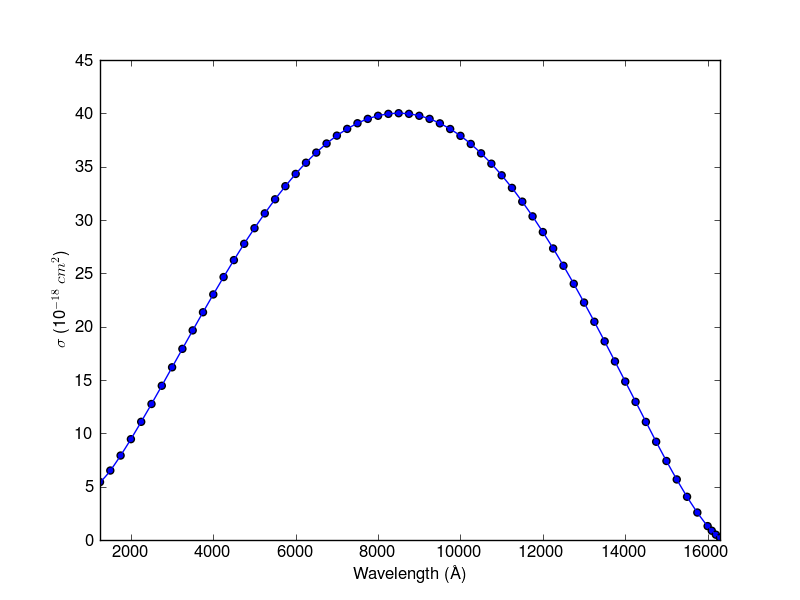
\includegraphics[width=80mm]{figs/boundfree_crosssection.png}
\caption{\label{fig:bfcrosssection}The bound-free photo-detachment
cross-section of \h\. Tabulated values calculated
by \cite{wishart1979} are given as open circles with a cubic spline
interpolation shown as the line connecting the points.  The calculated
cross-sections span from near infrared (at the wavelengths where photon
energies are sufficiently high to ionize the least bound electron
of \h) to near ultraviolet. As shown, photon energy increases along
the x-axis from right to left.}
\end{figure}
